\documentclass[tikz,border=10pt]{standalone}
\usepackage{tikz}
\usepackage{amsmath}
\usepackage{amssymb}
\usetikzlibrary{arrows.meta, calc, decorations.pathreplacing}

\begin{document}

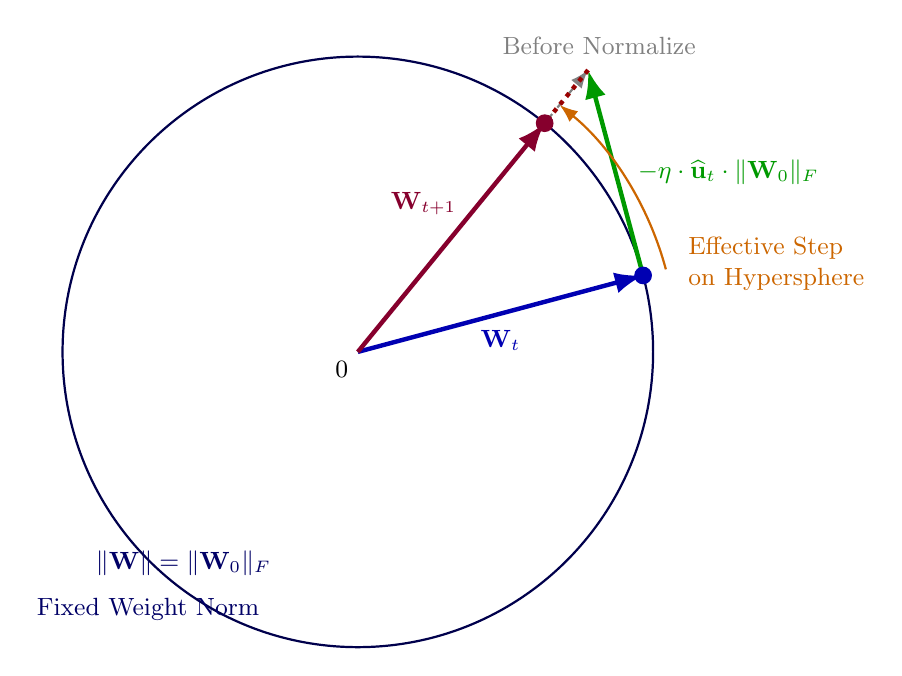
\begin{tikzpicture}[>=Latex, scale=1.5, font=\small]

    % --- 1. Define Coordinates ---
    % Hyperball Optimizer: W_{t+1} = Normalize(W_t - η·Normalize(u_t)·||W_0||_F) ||W_0||_F
    % Weights stay on a fixed hypersphere of radius ||W_0||_F
    
    \coordinate (O) at (0,0); % Origin
    \def\R{2.5} % Radius of the sphere (||W_0||_F - fixed!)
    \def\ang{15} % Angle of W_t

    % Extra radius for the effective-step arc
    \pgfmathsetmacro{\Rextra}{\R+0.2}

    % W_t coordinate (on the sphere)
    \coordinate (Wt) at (\ang:\R);
    
    % Normalized gradient direction (perpendicular-ish to W_t for visualization)
    % The update: -η · Normalize(u_t) · ||W_0||_F
    \def\stepLen{1.8} % η · ||W_0||_F
    \def\gradAng{105} % Direction of -Normalize(u_t) for illustration
    
    % Intermediate point (before normalization)
    \coordinate (Wt_inter) at ($ (Wt) + ({\gradAng}:\stepLen) $);
    
    % W_{t+1} after normalization (project back onto sphere)
    \pgfmathanglebetweenpoints{\pgfpointanchor{O}{center}}{\pgfpointanchor{Wt_inter}{center}}
    \let\angNew\pgfmathresult
    \coordinate (Wt_next) at (\angNew:\R);

    % --- 2. Draw Sphere (Fixed Radius) ---
    % Solid circle for Fixed Weight Norm ||W_0||_F
    \draw[thick, blue!30!black] (O) circle (\R);
    
    % --- 3. Main Vectors ---
    
    % W_t (Blue) - on the sphere
    \draw[->, ultra thick, blue!70!black] (O) -- (Wt) 
        node[midway, below, yshift=-2pt, text=blue!70!black] {$\mathbf{W}_t$};
    
    % Normalized Gradient Update (Green) - unit direction scaled by η||W_0||_F
    \draw[->, ultra thick, green!60!black] (Wt) -- (Wt_inter) 
        node[midway, right, xshift=4pt, yshift=0pt, align=left, text=green!60!black] 
        {$-\eta \cdot \widehat{\mathbf{u}}_t \cdot \|\mathbf{W}_0\|_F$};

    % Intermediate point (dashed, off-sphere)
    \draw[->, thick, dashed, gray] (O) -- (Wt_inter) 
        node[above, xshift=4pt, yshift=2pt, text=gray] {Before Normalize};
    
    % Projection back to sphere (dotted line)
    \draw[dotted, ultra thick, red!60!black] (Wt_inter) -- (Wt_next);

    % W_{t+1} (Purple) - back on the sphere
    \draw[->, ultra thick, purple!70!black] (O) -- (Wt_next) 
        node[midway, above, yshift=4pt, xshift=-10pt, text=purple!70!black] {$\mathbf{W}_{t+1}$};
    
    % Mark W_{t+1} point on the circle
    \filldraw[purple!70!black] (Wt_next) circle (2pt);
    
    % Mark W_t point on the circle
    \filldraw[blue!70!black] (Wt) circle (2pt);

    % --- 4. Effective Step Arc ---
    
    % Arc showing the effective angular step on the sphere
    \draw[thick, ->, orange!80!black] ({\ang}:\Rextra) arc (\ang:\angNew:\Rextra);
    \node[right, align=left, orange!80!black] at ($ (Wt) + (0.3, 0.1) $) {Effective Step\\on Hypersphere};

    % --- 5. Labels and Annotations ---
    
    % Fixed Norm Label
    \node[anchor=north west, blue!40!black] at (-\R-0.3, -\R+0.5) {Fixed Weight Norm};
    \node[anchor=north west, blue!40!black] at (-\R+0.2, -\R+0.9) {$\|\mathbf{W}\| = \|\mathbf{W}_0\|_F$};

    % Origin
    \node[below left] at (O) {$0$};

\end{tikzpicture}

\end{document}
